\documentclass[14pt]{article}

\usepackage[utf8x]{inputenc}
\usepackage[russian]{babel}
\usepackage{graphicx}
\graphicspath{{images/}}
\DeclareGraphicsExtensions{.pdf,.png,.jpg}

\usepackage{amsmath}
\usepackage{pgfplots}

\usepackage{geometry} % Меняем поля страницы
\geometry{left=2cm}% левое поле
\geometry{right=1.5cm}% правое поле
\geometry{top=2cm}% верхнее поле
\geometry{bottom=2cm}% нижнее поле

\renewcommand{\theenumi}{\arabic{enumi}}
\renewcommand{\labelenumi}{\arabic{enumi}}
\renewcommand{\theenumii}{.\arabic{enumii}}
\renewcommand{\labelenumii}{\arabic{enumi}.\arabic{enumii}.}
\renewcommand{\theenumiii}{.\arabic{enumiii}}
\renewcommand{\labelenumiii}{\arabic{enumi}.\arabic{enumii}.\arabic{enumiii}.}

\begin{document}
\begin{titlepage}
	\begin{center}
		\fontsize{18pt}{20pt}\selectfont
		\textbf{Работа 3.5.1.}	
	
		\vspace{5cm}
		\fontsize{24pt}{25pt}\selectfont
		Изучение плазмы газового разряда в неоне
	\end{center}
	\begin{flushright}
		\fontsize{18pt}{20pt}\selectfont
		\vspace{14cm}
		\hspace{-3cm}
		\textit{Корнеев Е.С.}
	\end{flushright}		
\end{titlepage}

\begin{center}
	\fontsize{16pt}{18pt}\selectfont	
	Изучение плазмы газового разряда в неоне
\end{center}


\fontsize{14pt}{16pt}\selectfont
\vspace{1cm}
\textbf{Цель работы:} изучение вольт-амперной характеристики тлеющего разряда; изучение свойств плазмы методом зондовых характеристик.

\vspace{0.5cm}
\textbf{Оборудование:} стеклянная газоразрядная трубка, наполненная изотопом неона, высоковольтный источник питания, источник питания постоянного тока, делитель напряжения, резистор, потенциометр, амперметры, вольтметры, переключатели. 

\vspace{1cm}
\textbf{Экспериментальная установка.} Схема установки для исследования плазмы газового разряда в неоне представлена на рисунке 1. Стеклянная трубка имеет холодный (ненакаливаемый) полый катод, три анода и геттерный узел - специальный баллон, на внутреннюю поверхность которого напылена газопоглощающая пленка (геттер).Трубка наполнена изотопом неона $^{22}$Ne при давлении 2 мм.рт.ст. Катод и один из анодов (I или II) с помощью переключателя П$_1$ подключается через балластный резистор 
$R_\text{б}~(\approx 450 \text{кОм})$ к регулируемому высоковольтному источнику питания (ВИП) с выходным напряжением до 3кВ. 

\begin{figure}[h!]
	\center{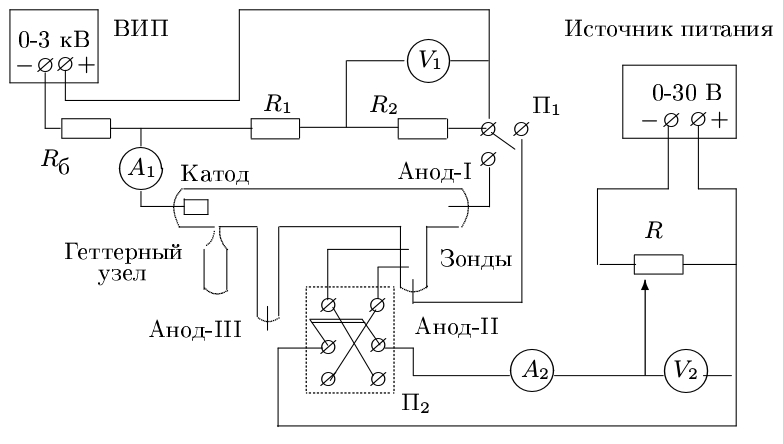
\includegraphics[width = 15cm]{1}}
	\caption{Схема установки}
	\label{fig:image}
\end{figure}

При подключении к ВИП анода-I между ним и катодом возникает газовый разряд. Ток разряда измеряется миллиамперметром $A_1$, а падение напряжения на разрядной трубке - цифровым вольтметром $V_1$ (В7-38), подключенным к трубке через высокоомный (25 МОм) делитель напряжения с коэффициентом $(R_1 + R_2)/R_2 = 10$.

При подключении к ВИП анода-II разряд возникает в пространстве между катодом и анодом-II, где находится двойной зонд, используемый для диагностики плазмы положительного столба. Зонды изготовлены из молибденовой проволоки диаметром $d = 0.2$ мми имеют длину $l = 5.2$ мм. Они подключены к источнику питания (0-30 В) через потенциометр $R$. Переключатель П$_2$ позволяет изменять полярность напряжения на зондах. Величина напряжения на зондах изменяется с помощью дискретного переключателя "$V$" выходного напряжения источника питания и потенциометра $R$, а измеряется вольтметром $V_2$. Для измерения зондового тока используется микроамперметр $A_2$. 

Анод-III в нашей работе не используется. 

\newpage

\textbf{Ход работы.}

Снимем ВАХ разряда:

\begin{center}
\begin{tabular}{|c|c|c|c|c|c|c|c|c|c|c|c|}
\hline
$U_1$, В&$I$, дел&$I$, мА&$U_1$, В&$I$, дел&$I$, мА\\
\hline
30,3&36&1,44&24,2&51&2,04\\
\hline
31,3&34&1,36&23,8&53&2,12\\
\hline
30,8&35&1,40&23,3&55&2,20\\
\hline
31,4&33&1,32&22,7&58&2,32\\
\hline
31,8&32&1,28&22,2&61&2,44\\
\hline
32,0&31&1,24&21,7&64&2,56\\
\hline
32,2&30&1,20&21,4&67&2,68\\
\hline
32,3&29&1,16&21,0&70&2,80\\
\hline
32,4&27&1,08&20,8&73&2,92\\
\hline
32,6&24&0,96&20,6&76&3,04\\
\hline
32,7&23&0,92&20,4&79&3,16\\
\hline
33,0&21&0,84&20,1&82&3,28\\
\hline
33,3&19&0,76&20,0&85&3,40\\
\hline
33,6&17&0,68&19,8&88&3,52\\
\hline
33,9&15&0,60&19,7&91&3,64\\
\hline
34,4&13&0,52&19,5&94&3,76\\
\hline
29,8&37&1,48&19,4&97&3,88\\
\hline
29,2&38&1,52&19,4&100&4,00\\
\hline
28,8&39&1,56&19,3&105&4,20\\
\hline
27,4&41&1,64&19,2&110&4,40\\
\hline
26,5&43&1,72&19,2&115&4,60\\
\hline
25,6&45&1,80&19,0&120&4,80\\
\hline
25,2&47&1,88&19,0&125&5,00\\
\hline
24,7&49&1,96&&&\\
\hline
\end{tabular}
\end{center}

\vspace{1cm}
Погрешность $I$ примем равной $1/2$ дел, то есть $0.02$ мА, так как измерения проводились при помощи прибора со шкалой, имеющей 150 делений, в режиме с $I_{max} = 6$мА. Погрешность $U$ примем равной 0.1В, так как в этих пределах значение напряжения оставалось постоянным. При данном масштабе и <<размахе>> измерений эти погрешности оказываются слишком маленькими, чтобы их было видно на графике.

\begin{tikzpicture}
\begin{axis}[
	height = 10cm,
	width  = 15cm,
	every axis y label/.style={at = {(ticklabel cs: 0.5)}, rotate = 90, anchor = near ticklabel},
	xlabel = {$U$, В},
	ylabel = {$I$, дел},
	grid   = major,
]
\addplot+[
	only marks,
	error bars/.cd, 
	y dir = both, y explicit,
	x dir = both, x explicit,
	]
coordinates{
	(30.3,  36)
	(31.1,  34)
	(30.8,  35)
	(31.4,  33)
	(31.8,  32)
	(32.0,  31)
	(32.2,  30)
	(32.3,  29)
	(32.4,  27)
	(32.6,  24)
	(32.7,  23)
	(33.0,  21)
	(33.3,  19)
	(33.6,  17)
	(33.9,  15)
	(34.4,  13)
	
	(29.8,  37)
	(29.2,  38)
	(28.8,  39)
	(27.4,  41)
	(26.5,  43)
	(25.6,  45)
	(25.2,  47)
	(24.7,  49)
	(24.2,  51)
	(23.8,  53)
	(23.3,  55)
	(22.7,  58)
	(22.2,  61)
	(21.7,  64)
	(21.4,  67)
	(21.0,  70)
	
	(20.8,  73)
	(20.6,  76)
	(20.4,  79)
	(20.1,  82)
	(20.0,  85)
	(19.8,  88)
	(19.7,  91)
	(19.5,  94)
	(19.4,  97)
	(19.4, 100)
	(19.3, 105)
	(19.2, 110)
	(19.2, 115)
	(19.0, 120)
	(19.0, 125)
};

\addplot+[
	mark  = none,
	color = black	
	]
coordinates{
	(33.4,   0)
	(31.9,  40)
};

\end{axis}
\end{tikzpicture}

\vspace{1cm}
Проведем касательную в месте максимального угла наклона ВАХа. Получим:
$$
	R_{max} = -446~\text{Ом}
$$
Погрешность случайную оценим по МНК:
$$
	\sigma_\text{случ} = 30~\text{Ом}
$$
Приборной погрешностью на фоне случайной можно пренебречь. Таким образом:
$$
	R_{max} = (-450 \pm 30)~\text{Ом}
$$

\newpage
Снимем зондовые характеристики и построим соответствующие графики. Приборная погрешность $U$ по-прежнему будет равна $0.1$ В, погрешность же тока примем равной единице последнего разряда, то есть $0.1$ мкА.

\begin{center}
\begin{tabular}{|c|c|c|c|c|c|c|c|c|c|c|c|}
\hline
\multicolumn{2}{|c|}{$I = 5.0$ мА}&\multicolumn{2}{|c|}{$I = 3.0$ мА}&\multicolumn{2}{|c|}{$I = 1.5$ мА}\\
\hline
$U_2$, В&$I_2$, мкА&$U_2$, В&$I_2$, мкА&$U_2$, В&$I_2$, мкА\\
\hline
25,0&118,4&25,2&50,8&25,2&24,2\\
\hline
22,5&115,8&22,1&49,0&22,0&23,3\\
\hline
20,0&113,2&19,1&47,3&19,0&22,6\\
\hline
17,5&110,5&16,0&45,5&16,0&21,8\\
\hline
15,0&107,3&14,0&44,1&14,0&21,3\\
\hline
12,5&101,9&12,0&41,9&12,0&20,4\\
\hline
10,1&94,4&10,0&38,4&10,0&19,0\\
\hline
8,0&85,7&8,1&33,1&8,0&16,3\\
\hline
6,0&74,2&6,0&25,0&6,0&12,6\\
\hline
4,0&59,2&4,0&14,9&4,1&7,5\\
\hline
2,0&41,6&2,0&2,6&2,0&0,0\\
\hline
1,5&35,0&1,5&-1,0&1,5&-0,8\\
\hline
1,0&29,0&1,0&-4,3&1,0&-2,5\\
\hline
0,5&23,8&0,5&-7,7&0,5&-4,4\\
\hline
-25,1&-89,0&-25,1&-68,8&-25,2&-37,1\\
\hline
-22,0&-90,0&-22,0&-66,6&-22,0&-35,7\\
\hline
-19,0&-88,8&-19,0&-64,5&-19,0&-34,4\\
\hline
-16,0&-85,8&-16,0&-62,5&-16,1&-33,2\\
\hline
-14,0&-82,0&-14,0&-60,9&-14,0&-32,3\\
\hline
-12,0&-76,5&-12,0&-58,8&-12,0&-31,2\\
\hline
-10,0&-68,7&-10,0&-55,9&-10,0&-29,7\\
\hline
-8,1&-58,0&-8,1&-51,7&-8,0&-27,8\\
\hline
-6,0&-43,0&-6,0&-45,0&-6,0&-24,4\\
\hline
-4,0&-25,0&-4,0&-36,2&-4,1&-19,9\\
\hline
-2,1&-5,2&-2,0&-24,6&-2,0&-13,6\\
\hline
-1,5&-1,5&-1,5&-21,3&-1,5&-11,9\\
\hline
-1,0&7,0&-1,0&-18,2&-1,0&-10,2\\
\hline
-0,5&12,1&-0,5&-14,6&-0,5&-8,3\\
\hline
\end{tabular}
\end{center}

\newpage
Построим все характеристики на одном графике:

\vspace{1cm}
\begin{tikzpicture}
\begin{axis}[
	height = 10cm,
	width  = 15cm,
	every axis y label/.style={at = {(ticklabel cs: 0.5)}, rotate = 90, anchor = near ticklabel},
	xlabel = {$U$, В},
	ylabel = {$I$, мкА},
	grid   = major,
]

\addplot+[
	smooth
	]
coordinates{
	( 25.0, 118.4)
	( 22.5, 115.8)
	( 20.0, 113.2)
	( 17.5, 110.5)
	( 15.1, 107.3)
	( 12.5, 101.9)
	( 10.1,  94.4)
	( 8.0 ,  85.7)
	( 6.0 ,  74.2)
	( 4.0 ,  59.2)
	( 2.0 ,  41.6)
	( 1.5 ,  35.0)
	( 1.0 ,  29.3)
	( 0.5 ,  23.8)
	
	(-25.1, -89.0)
	(-22.0, -90.0)
	(-19.0, -88.8)
	(-16.0, -85.8)
	(-14.0, -82.0)
	(-12.0, -76.5)
	(-10.0, -68.7)
	( -8.1, -58.0)
	( -6.0, -43.0)
	( -4.0, -25.0)
	( -2.1,  -5.2)
	( -1.5,  -1.5)
	( -1.0,     7)
	( -0.5,  12.1)
};

\addplot+[
	smooth
	]
coordinates{
	( 25.2,  50.8)
	( 22.1,  49.0)
	( 19.1,  47.3)
	( 16.0,  45.5)
	( 14.0,  44.1)
	( 12.0,  41.9)
	( 10.0,  38.4)
	( 8.0 ,  33.1)
	( 6.0 ,  25.0)
	( 4.0 ,  14.9)
	( 2.0 ,   2.6)
	( 1.5 ,  -1.0)
	( 1.0 ,  -4.3)
	( 0.5 ,  -7.7)
	
	(-25.1, -68.8)
	(-22.0, -66.6)
	(-19.0, -64.6)
	(-16.0, -62.5)
	(-14.0, -60.9)
	(-12.0, -58.8)
	(-10.0, -55.9)
	( -8.1, -51.7)
	( -6.0, -45.0)
	( -4.0, -36.2)
	( -2.0, -24.6)
	( -1.5, -21.3)
	( -1.0, -18.2)
	( -0.5, -14.6)
};

\addplot+[
	smooth
	]
coordinates{
	( 25.2,  24.2)
	( 22.0,  23.3)
	( 19.0,  22.6)
	( 16.0,  21.8)
	( 14.0,  21.3)
	( 12.0,  20.4)
	( 10.0,  19.0)
	( 8.0 ,  16.3)
	( 6.0 ,  12.6)
	( 4.1 ,   7.5)
	( 2.0 ,   0.0)
	( 1.5 ,  -0.8)
	( 1.0 ,  -2.5)
	( 0.5 ,  -4.4)
	
	(-25.1, -37.1)
	(-22.0, -35.7)
	(-19.0, -34.4)
	(-16.0, -33.2)
	(-14.0, -32.3)
	(-12.0, -31.2)
	(-10.0, -29.7)
	( -8.1, -27.8)
	( -6.0, -24.4)
	( -4.0, -19.9)
	( -2.0, -13.6)
	( -1.5, -11.9)
	( -1.0, -10.2)
	( -0.5,  -8.3)
};

\end{axis}
\end{tikzpicture}


\newpage
Соответствующие зондовые характеристики представлены далее. Синим цветом выделены полученные значения, красным - центрированные.

\vspace{0.5cm}
$I = 5.0$ мкА

\begin{tikzpicture}
\begin{axis}[
	height = 10cm,
	width  = 15cm,
	every axis y label/.style={at = {(ticklabel cs: 0.5)}, rotate = 90, anchor = near ticklabel},
	xlabel = {$U$, В},
	ylabel = {$I$, мкА},
	grid   = major,
]
\addplot+[
	smooth
	]
coordinates{
	( 25.0, 118.4)
	( 22.5, 115.8)
	( 20.0, 113.2)
	( 17.5, 110.5)
	( 15.1, 107.3)
	( 12.5, 101.9)
	( 10.1,  94.4)
	( 8.0 ,  85.7)
	( 6.0 ,  74.2)
	( 4.0 ,  59.2)
	( 2.0 ,  41.6)
	( 1.5 ,  35.0)
	( 1.0 ,  29.3)
	( 0.5 ,  23.8)
	
	(-25.1, -89.0)
	(-22.0, -90.0)
	(-19.0, -88.8)
	(-16.0, -85.8)
	(-14.0, -82.0)
	(-12.0, -76.5)
	(-10.0, -68.7)
	( -8.1, -58.0)
	( -6.0, -43.0)
	( -4.0, -25.0)
	( -2.1,  -5.2)
	( -1.5,  -1.5)
	( -1.0,     7)
	( -0.5,  12.1)
};

% -15 :)

\addplot+[
	color = red,
	smooth
	]
coordinates{
(25, 103.4)
(22.5, 100.8)
(20, 98.2)
(17.5, 95.5)
(15.1, 92.3)
(12.5, 86.9)
(10.1, 79.4)
(8, 70.7)
(6, 59.2)
(4, 44.2)
(2, 26.6)
(1.5, 20)
(1, 14.3)
(0.5, 8.8)
(-0.5, -2.9)
(-1, -8)
(-1.5, -16.5)
(-2.1, -20.2)
(-4, -40)
(-6, -58)
(-8.1, -73)
(-10, -83.7)
(-12, -91.5)
(-14, -97)
(-16, -100.8)
(-19, -103.8)
(-22, -105)
(-25.1, -104)
};

\end{axis}
\end{tikzpicture}

\vspace{0.5cm}
$I = 3.0$ мкА

\begin{tikzpicture}
\begin{axis}[
	height = 10cm,
	width  = 15cm,
	every axis y label/.style={at = {(ticklabel cs: 0.5)}, rotate = 90, anchor = near ticklabel},
	xlabel = {$U$, В},
	ylabel = {$I$, мкА},
	grid   = major,
]
\addplot+[
	smooth
	]
coordinates{
	( 25.2,  50.8)
	( 22.1,  49.0)
	( 19.1,  47.3)
	( 16.0,  45.5)
	( 14.0,  44.1)
	( 12.0,  41.9)
	( 10.0,  38.4)
	( 8.0 ,  33.1)
	( 6.0 ,  25.0)
	( 4.0 ,  14.9)
	( 2.0 ,   2.6)
	( 1.5 ,  -1.0)
	( 1.0 ,  -4.3)
	( 0.5 ,  -7.7)
	
	(-25.1, -68.8)
	(-22.0, -66.6)
	(-19.0, -64.6)
	(-16.0, -62.5)
	(-14.0, -60.9)
	(-12.0, -58.8)
	(-10.0, -55.9)
	( -8.1, -51.7)
	( -6.0, -45.0)
	( -4.0, -36.2)
	( -2.0, -24.6)
	( -1.5, -21.3)
	( -1.0, -18.2)
	( -0.5, -14.6)
};

% +10

\addplot+[
	color = red,
	smooth
	]
coordinates{
(25.2, 60.8)
(22.1, 59)
(19.1, 57.3)
(16, 55.5)
(14, 54.1)
(12, 51.9)
(10, 48.4)
(8, 43.1)
(6, 35)
(4, 24.9)
(2, 12.6)
(1.5, 9)
(1, 5.7)
(0.5, 2.3)
(-0.5, -4.6)
(-1, -8.2)
(-1.5, -11.3)
(-2, -14.6)
(-4, -26.2)
(-6, -35)
(-8.1, -41.7)
(-10, -45.9)
(-12, -48.8)
(-14, -50.9)
(-16, -52.5)
(-19, -54.6)
(-22, -56.6)
(-25.1, -58.8)
};

\end{axis}
\end{tikzpicture}

\vspace{1cm}
$I = 1.5$ мкА

\begin{tikzpicture}
\begin{axis}[
	height = 10cm,
	width  = 15cm,
	every axis y label/.style={at = {(ticklabel cs: 0.5)}, rotate = 90, anchor = near ticklabel},
	xlabel = {$U$, В},
	ylabel = {$I$, мкА},
	grid   = major,
]
\addplot+[
	smooth
	]
coordinates{
	( 25.2,  24.2)
	( 22.0,  23.3)
	( 19.0,  22.6)
	( 16.0,  21.8)
	( 14.0,  21.3)
	( 12.0,  20.4)
	( 10.0,  19.0)
	( 8.0 ,  16.3)
	( 6.0 ,  12.6)
	( 4.1 ,   7.5)
	( 2.0 ,   0.0)
	( 1.5 ,  -0.8)
	( 1.0 ,  -2.5)
	( 0.5 ,  -4.4)
	
	(-25.1, -37.1)
	(-22.0, -35.7)
	(-19.0, -34.4)
	(-16.0, -33.2)
	(-14.0, -32.3)
	(-12.0, -31.2)
	(-10.0, -29.7)
	( -8.1, -27.8)
	( -6.0, -24.4)
	( -4.0, -19.9)
	( -2.0, -13.6)
	( -1.5, -11.9)
	( -1.0, -10.2)
	( -0.5,  -8.3)
};

% +6 

\addplot+[
	color = red,
	smooth
	]
coordinates{
(-25.1, -31.1)
(-22, -29.7)
(-19, -28.4)
(-16, -27.2)
(-14, -26.3)
(-12, -25.2)
(-10, -23.7)
(-8.1, -21.8)
(-6, -18.4)
(-4, -13.9)
(-2, -7.6)
(-1.5, -5.9)
(-1, -4.2)
(-0.5, -2.3)
(0.5, 1.6)
(1, 3.5)
(1.5, 5.2)
(2, 6)
(4.1, 13.5)
(6, 18.6)
(8, 22.3)
(10, 25)
(12, 26.4)
(14, 27.3)
(16, 27.8)
(19, 28.6)
(22, 29.3)
(25.2, 30.2)
};

\end{axis}
\end{tikzpicture}

\vspace{1cm}
Сведем в таблицу значения $I_{i\text{н}}$, $\frac{dI}{dU}|_{U = 0}$ и их погрешностей для различных значений $I$:

\begin{center}
\begin{tabular}{|c|c|c|c|c|c|c|c|c|c|c|c|c|c|}
\hline
$I$, мА		&	$I_{i\text{н}}$, мкА	&	$\sigma_{I_{i\text{н}}}$, мкА	&	$\frac{dI}{dU}|_{U = 0}$, мкА/В	&	$\sigma_{\frac{dI}{dU}|_{U = 0}}$, мкА/В	\\
\hline
5.0			&	77						&	2								&	11.6								&	0.3											\\
\hline
3.0			&	46						&	2								&	6.8									&	0.4											\\
\hline
1.5			&	24						&	2								&	3.6									&	0.3											\\
\hline
\end{tabular}
\end{center}

\vspace{1cm}
Теперь определим энергию электронов по формуле
$$
	E = kT = \frac{1}{2}\frac{eI_{i\text{н}}}{\frac{dI}{dU}|_{U = 0}} = 3.34~\text{эВ}
$$
Погрешность определим, считая $E = f(I_{i\text{н}}, \frac{dI}{dU}|_{U = 0})$, а также найдя отклонения значений в серии экспериментов от среднего. Получим:
$$
	E = (3.34 \pm 0.04)~\text{эВ}
$$

\vspace{1cm}
Зная $E$, можно определить $n_e$:
$$
	I_{i\text{н}} = 0.4n_eeS\sqrt{\frac{2kT}{m_i}} \Rightarrow n_e = 2.5\frac{I_{i\text{н}}}{eS}\sqrt{\frac{m_i}{2kT}},
$$
\noindent где $S = \pi ld$, $l = 5.2$ мм, $d = 0.2$ мм, $m_i = 22\cdot1.66\cdot10^{-27}$ кг. Получим:

\begin{center}
\begin{tabular}{|c|c|c|c|c|c|c|c|c|c|c|c|c|c|}
\hline
$I_{i\text{н}}$, мкА	&	$n_e$, м$^{-3}\cdot10^{15}$	&	$\sigma_{n_e}$, м$^{-3}\cdot10^{15}$	\\
\hline
77						&	68							&	2										\\
\hline
46						&	41							&	2										\\
\hline
24						&	21							&	2										\\
\hline
\end{tabular}
\end{center}

\vspace{1cm}
Построим графики зависимостей $T(I_p)$ и $n_e(I_p)$:

\vspace{1cm}

\begin{tikzpicture}
\begin{axis}[
	height = 8cm,
	width  = 15cm,
	every axis y label/.style={at = {(ticklabel cs: 0.5)}, rotate = 90, anchor = near ticklabel},
	xlabel = {$I_p$, мА},
	ylabel = {$T$, K$\cdot 10^3$},
	grid   = major,
]
\addplot+[
	only marks,
	error bars/.cd, 
	y dir = both, y explicit,
	x dir = both, x explicit
	]
coordinates{
	(1.5, 38.6)	+-	(0.1, 0.5)
	(3.0, 39.2)	+-	(0.1, 0.5)
	(5.0, 38.4)	+-	(0.1, 0.5)
};

\addplot+[
	mark  = none,
	color = blue
	]
coordinates{
	(1.2, 38.75)
	(5.3, 38.75)
};

\end{axis}
\end{tikzpicture}

\hspace*{0.2cm}
\begin{tikzpicture}
\begin{axis}[
	height = 8cm,
	width  = 15cm,
	every axis y label/.style={at = {(ticklabel cs: 0.5)}, rotate = 90, anchor = near ticklabel},
	xlabel = {$I_p$, мА},
	ylabel = {$n_e$, м$^{-3}\cdot10^{15}$},
	grid   = major,
]
\addplot+[
	smooth,
	error bars/.cd, 
	y dir = both, y explicit,
	x dir = both, x explicit
	]
coordinates{
	(1.5, 21)	+-	(0.1, 1)
	(3.0, 41)	+-	(0.1, 2)
	(5.0, 68)	+-	(0.1, 2)
};

\end{axis}
\end{tikzpicture}

\newpage
Найдем плазменную частоту колебаний электронов:
$$
	\omega_p = \sqrt{\frac{n_ee^2}{\epsilon_0m_e}}
$$

\begin{center}
\begin{tabular}{|c|c|c|c|c|c|c|c|c|c|c|c|c|c|}
\hline
$n_e$, м$^{-3}\cdot10^{15}$	&	$\omega_p$, $c^{-1}\cdot 10^6$	&	$\sigma_{\omega_p}$, $c^{-1}\cdot 10^6$	\\
\hline
21							&	260								&	20											\\
\hline
41							&	360								&	20 											\\
\hline
68							&	480								&	20											\\
\hline
\end{tabular}
\end{center}

\vspace{1cm}
А также дебаевский радиус:
$$
	r_D = \sqrt{\frac{kT}{4\pi ne^2}}
$$

\begin{center}
\begin{tabular}{|c|c|c|c|c|c|c|c|c|c|c|c|c|c|}
\hline
$n_e$, м$^{-3}\cdot10^{15}$	&	$r_D$, м$^{-4}$		&	$\sigma_{r_D}$, м$^{-4}$	\\
\hline
21							&	2.61				&	0.13						\\
\hline
41							&	1.86				&	0.09						\\
\hline
68							&	1.45				&	0.08						\\
\hline
\end{tabular}
\end{center}

\vspace{1cm}
Зная дебаевский радиус, можно найти число электронов в дебаевской сфере:
$$
	N = \frac{4}{3}\pi r_D^3 n_e
$$

\begin{center}
\begin{tabular}{|c|c|c|c|c|c|c|c|c|c|c|c|c|c|}
\hline
$n_e$, м$^{-3}\cdot10^{15}$	&	$N$		&	$\sigma_N$	\\
\hline
21							&	1560	&	80			\\
\hline
41							&	1120	&	60			\\
\hline
68							&	870		&	40			\\
\hline
\end{tabular}
\end{center}

\vspace{1cm}
Оценим степень ионизации плазмы:
$$
	\alpha = \frac{n_ekT}{P},
$$
где $P = 1$ мбар. Получим:

\begin{center}
\begin{tabular}{|c|c|c|c|c|c|c|c|c|c|c|c|c|c|}
\hline
$n_e$, м$^{-3}\cdot10^{15}$	&	$\alpha, 10^{-7}$ 	&	$\sigma_\alpha$	\\
\hline
21							&	8.7					&	0.5				\\
\hline
41							&	17.0				&	0.9				\\
\hline
68							&	28.2				&	1.5				\\
\hline
\end{tabular}
\end{center}

\newpage
Таким образом, в данной лабораторной работе мы изучили газовый разряд и такие свойства плазмы, как концентрация электронов, плазменная частота колебаний электронов и дебаевский радиус при помощи двойного зонда, а также построили ВАХ тлеющего разряда.


\end{document}

